%-------------------------------------------------------------------------------
%-------------------------------------------------------------------------------
\section{Déterminant} \label{sec:LinAlg-Det}
%-------------------------------------------------------------------------------
%-------------------------------------------------------------------------------

\begin{definition*}[Matrice inversible]
  Une matrice $A \in \Mcal_n$ est dite inversible si la solution $x \in \Rbb^n$ du système linéaire $A x = y$ est unique quelque soit le vecteur $y \in \Rbb$.
\end{definition*}

Il existe alors une unique matrice $B$ telle que 
$$
AB = BA = I_n
$$
et notée $A^{-1} = B$. La solution de $Ax = y$ est alors $x = A^{-1} y$.

On cherche à déterminer à quelle condition une matrice carrée $A$ est inversible.

%-------------------------------------------------------------------------------
%-------------------------------------------------------------------------------
\subsection{Matrices $2 \times 2$} 
%-------------------------------------------------------------------------------

\begin{exercise*}
  Donner une condition nécessaire et suffisante sur $(a, b, c, d)$ pour que 
  $$
  A = \left[\begin{array}{cc} a & b \\ c & d \end{array} \right]
  $$
  soit inversible et donner $A^{-1}$.
\end{exercise*}

\solution{Voir \cite{Lam20}, p 6.}

\begin{definition*}[1.2.2: Déterminant d'une matrice de $\Mcal_2$]
  Le déterminant de la matrice $A \in \Mcal_2$ est noté $\det(A)$ ou $|A|$ et vaut
  $$
  |A| = a_{11} a_{22} - a_{12} a_{21}.
  $$
\end{definition*}

Le déterminant d'une matrice de $\Mcal_2$ est une fonction continue qui s'annule ssi la matrice n'est pas inversible : on cherche à généraliser cette notion aux matrices de $\Mcal_n$.

\begin{exercise*} Montrer les égalités suivantes : 
  \begin{enumerate}
    \item transformation linéaire d'une colonne
    $$
    \left| \begin{array}{cc} \lambda a + a' & b \\ \lambda c + c' & d \end{array} \right|
    =
    \lambda \left| \begin{array}{cc} a & c \\ c & d \end{array} \right|
    +
    \left| \begin{array}{cc} a' & b \\ c ' & d \end{array} \right|
    $$
    \item interversion des deux colonnes
    $$
    \left| \begin{array}{cc} a & b \\ c & d \end{array} \right|
    =
    - \left| \begin{array}{cc} b & a \\ d & c \end{array} \right|.
    $$
  \end{enumerate}
\end{exercise*}

\solution{Directe}

\remark On a ainsi montré que, en considérant $\det(A)$ comme une fonction des deux vecteurs colonnes de $A$:
$$
x_1 = \left(\begin{array}{c}a \\c \end{array} \right), \quad
x_2 = \left(\begin{array}{c}b \\d \end{array} \right) \in \Rbb^2 =: E, \qquad
\begin{array}{r|rcl}
  \det : & E^2 & \mapsto & \Rbb \\
  & (x_1, x_2) & \rightarrow & ab - bc,
\end{array}
$$
cette fonction est linéaire par rapport à chacune des deux vecteurs $x_1$ et $x_2$ et 'alternée'.

%-------------------------------------------------------------------------------
%-------------------------------------------------------------------------------
\subsection{Déterminant de matrices $n \times n$} 
%-------------------------------------------------------------------------------

\begin{definition*}[Application $n$-linéaire]
  Soit $E$ un espace vectoriel et $f: E^n \mapsto \Rbb$. $f$ est dite $n$-linéaire si elle est linéaire par rapport à chacune des $n$ variables:
  $$
  \forall 1 \leq i \leq n: \quad
  f(u_1, \dots, \lambda u_i + v_i, \dots u_n) = \lambda f(u_1, \dots, u_i, \dots u_n) + f(u_1, \dots, v_i, \dots u_n).
  $$
\end{definition*}

\begin{definition*}[Application alternée]
  Soit $E$ un espace vectoriel et $f: E^n \mapsto \Rbb$. $f$ est dite alternée si elle prend la valeur opposée quand on permuted eux variables : 
  $$
  f(x_1, \dots x_i, \dots x_j, \dots x_n)
  =
  - f(x_1, \dots x_j, \dots x_i, \dots x_n).
  $$
\end{definition*}

\begin{theorem*}[1.2.5 Unicité du déterminant]
  Il n'existe qu'une seule application $\varphi: \Mcal_n \mapsto \Rbb$ qui soit $n$-linéaire, alternée et telle que $\varphi(I_n) = 1$. Cette application est appelée 'déterminant'. \\
  De plus
  \begin{enumerate}[($a$)]
   \item Pour toute $A \in \Mcal_n$: $\det(A) \neq 0 \Leftrightarrow A$ inversible;
   \item Pour toute $A$de $\Mcal_n$: $\det(A) = \det(A^\top)$;
   \item Pour toutes $A$ et $B$ de $\Mcal_n$: $\det(A B) = \det(B A) = \det(A) \det(B)$.
  \end{enumerate}
\end{theorem*}

\proof [Théorème 1.2.5]
% On ne démontre que la propriété ($a$).
% Par définition de l'inversibilité, $A$ est inversible ssi l'application
% $$
% \begin{array}{r|rcl}
%   f: & \Rbb^n & \mapsto & \Rbb^n\\
%     & x & \rightarrow & y = Ax
% \end{array}
% $$
% est une bijection (car alors tout vecteur $y$ de $\Rbb^n$ possède un antécédent $x$ dans $\Rbb^n$) et l'application $f$ est une bijection ssi elle transforme une base de $\Rbb^n$ en une base de $\Rbb^n$. On considère alors les deux implications
% \begin{itemize}
% \item $\det(A) \neq 0 \Rightarrow f$ bijective: par contraposée, si $f$ n'est pas une bijection, l'image d'une base est une famille liée, donc une des colonnes de $A$ est combinaison linéaire des autres, donc $|A| = 0$ par le lemme précédent.
% \item $f$ bijective $\Rightarrow \det(A) \neq 0$: 
% \todo{Utiliser \cite{GAJ94}, Thm 3 (p14), ii/.}
% \end{itemize}
\begin{enumerate}[\itemdot]
 \item Non faite en cours. 
 \item Voir par exemple \cite{GAJ94} (Thm 3, p14, ii/) ou \cite{Ser01} (prop 2.2.1, p16).
\end{enumerate}
\eproof

\remark Une conséquence de cette propriété est que, si $A$ est inversible, puisque $|I_n| = 1$,
$$
|A^{-1}| = |A|^{-1}.
$$

\begin{exercise*}[1.2.6 : déterminant d'une matrice diagonale]
  En utilisant seulement la $n$-linéarité et le fait que $|I_n| = 1$, montrer que 
  $$
  |\diag(\lambda_1, \dots \lambda_n)| = \prod_{i = 1}^n \lambda_i.
  $$
\end{exercise*}

\solution{
  On applique la $n$ linéarité à chacun des termes diagonaux de la matrice $\diag(\lambda_1, \dots \lambda_n)$ : 
  \begin{align*}
  |\diag(\lambda_1, \dots \lambda_n)| 
  & = \lambda_1 \times |\diag(1, \lambda_2, \dots \lambda_n)|
  = \lambda_1 \lambda_2 \times |\diag(1, 1, \lambda_3, \dots \lambda_n)| \\
  & = \lambda_1 \lambda_2 \dots \lambda_n \times |\diag(1, 1, \dots 1)|
  = \prod_{i=1}^n \lambda_i \times |I_n|.
  \end{align*}
}

\begin{lemma*}
  $|A| = 0$ dans les deux cas suivants :
  \begin{enumerate}[($i$)] 
  \item $A$ comporte une colonne nulle ;
  \item une colonne de $A$ est combinaison linéaire des autres.
  \end{enumerate}
\end{lemma*}

\proof[Lemme]
  \begin{enumerate}[($i$)] 
  \item La $n$-linéarité implique que, si la matrice $B$ est construite à partir de la matrice $A$ en multipliant une de ses colonnes par $\lambda$, on a $|B| = \lambda |A|$. La propriété s'obtient en prenant $\lambda = 0$.
  \item On commence par remarquer que le caractère alterné du déterminant implique qu'il est nulle pour une matice ayant deux colonnes égales puisque
  $$
  det(x_1, x_1, x_2,\dots, x_n) = -det(x_1, x_1, x_2,\dots, x_n)
  $$
  La $n$-linéarité implique donc que, si on ajoute une combinaison linéaire de toute les colonnes à l'une d'entre elle, le déterminant ne change pas. En effet
  \begin{align*}
    \det\left(x_1, \dots, x_{n-1}, x_n + \sum_{i=1}^{n-1} \lambda_i x_i\right)
    & = \det\left(x_1, \dots, x_{n-1}, x_n\right)
    + \sum_{i=1}^{n-1} \lambda_i \det\left(x_1, \dots, x_{n-1}, x_i\right)
  \end{align*}
  or, pour tout $i = 1, \dots n-1$, $ \det\left(x_1, \dots, x_i, \dots, x_{n-1}, x_i\right) = 0$. \\
  L'ajout d'une combinaison linéaire des autres colonnes à l'une d'entre elles ne change donc pas le déterminant (\cite{GAJ94}, Prop 12, p13). \\
  Le cas où une colonne est combinaison linéaire des autres correspond au cas ou $x_n = 0_n$, soit
  $$
  \det\left(x_1, \dots x_{n-1}, 0_n + \sum_{i=1}^{n-1} \lambda_i x_i\right)
  = \det\left(x_1, \dots, x_{n-1}, 0_n\right)
  = 0
  $$
  d'après le ($i$).
  \end{enumerate}
  (On peut noter que ($i$) est un cas particulier de ($ii$).)
\eproof

\begin{proposition*}
  \begin{equation} \label{eq:determinant}
    |A| = \sum_{\sigma \in \Scal_n} (-1)^{s(\sigma)} \prod_{i=1}^n a_{i, \sigma(i)} 
    \end{equation}
    où $\Scal$ est l'ensemble des permutation de $\{1, \dots n\}$ et $s(\sigma) \in \{-1, +1\}$ désigne la signature de la permutation $\sigma$. Cette formule est rarement utilisée en pratique (notamment parce que $|\Scal| = n!$), sauf pour $n=2$ ou $n=3$.
\end{proposition*}

\proof Non démontrée. \eproof.

\remark La propriété $|A| = |A^\top|$ entraîne que les propriétés du déterminant quant aux colonnes (forme alternée, multilinéarité) sont également vraies pour les lignes. 

\remark La propriété selon laquelle une matrice dont une colonne est combinaison linéaire des autres a un déterminant nul donne une intuition du lien entre nullité du déterminant et non inversibilité. En supposant que cette colonne soit la dernière, le calcul de $A e_n$ (où $e_n$ est le dernier vecteur de la basse canonique) montre que c'est une combinaison linéaire des vecteurs $A e_i$ pour $1 \leq i \leq n-1$ et les images des vecteurs de $\Rbb^n$ appartiennent toutes à un espace de dimension au plus $n-1$, ce qui interdit à $A$ d'être inversible.

\remark D'un point de vue géométrique, un déterminant peut être interprété comme un volume. Il existe notamment deux cas simples :
\begin{enumerate}
 \item Dimension 2 : faire le calcul
  Soit $x = (a, c)$ et $y = (b, d)$, la surface $S$ parallélograme de sommets $\{0, x, y, x+y\}$ est égale à la surface du rectangle de sommet supérieur droit $x+y$ privé des surface $(1)$, $(2)$, $(3)$ et $(4)$ : 
  $$
  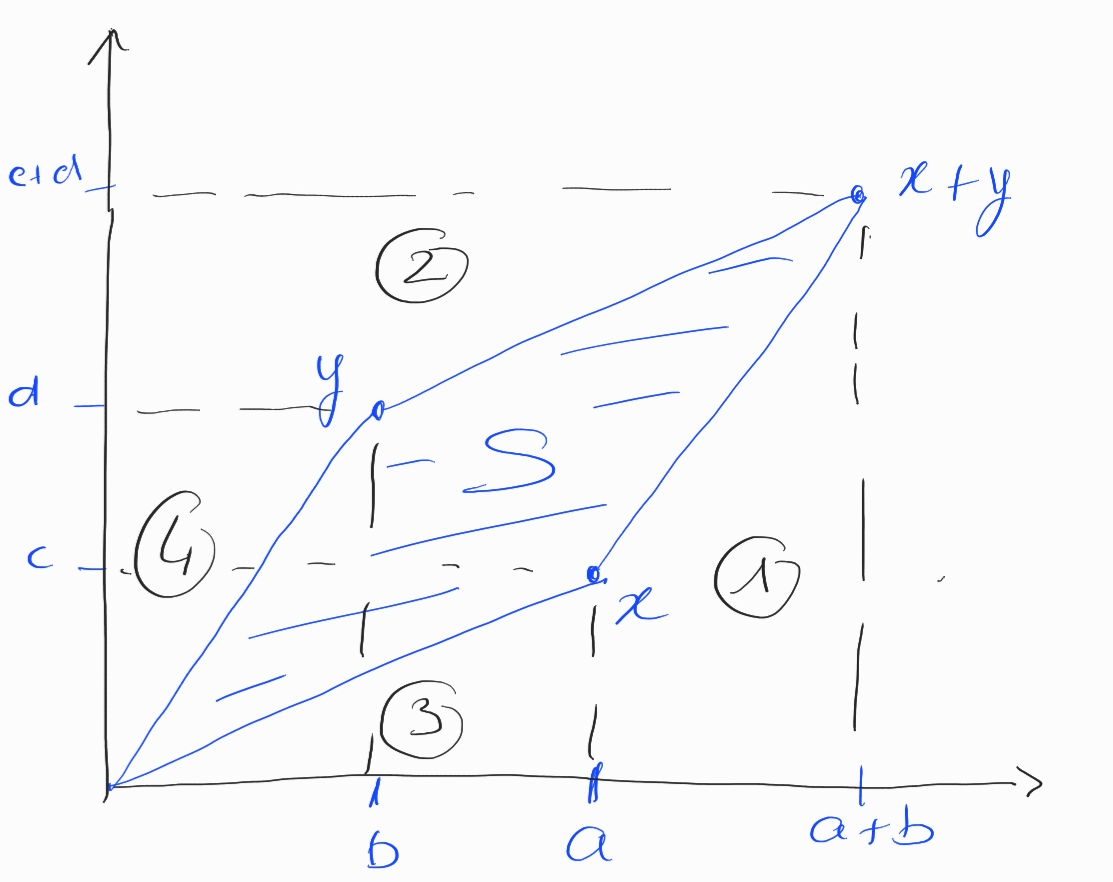
\includegraphics{DeterminantVolumeDimension2}
  $$
  soit
  \begin{align*}
    S 
    & = (a+b)(c+d) 
    - \underset{(1)}{\underbrace{b\left(c + \frac{d}2\right)}} 
    - \underset{(2)}{\underbrace{c\left(b + \frac{a}2\right)}} 
    - \underset{(3)}{\underbrace{\left(\frac{ac}2\right)}} 
    - \underset{(4)}{\underbrace{\left(\frac{bd}2\right)}} \\
    & = \dots = ad - bc.
  \end{align*}
 \item Dimension $n$ : matrice diagonale = volume d'un parallélépipède.
\end{enumerate}

%-------------------------------------------------------------------------------
%-------------------------------------------------------------------------------
\subsection{Calcul de déterminant de matrices $n \times n$} 
%-------------------------------------------------------------------------------

On s'intéresse ici au calcul effectif d'un déterminant.

\begin{proposition*}[Déterminant par blocs]
  Soit $A \in \Mcal_{n,n}$ de la forme
  $$
  A = \left[\begin{array}{cc}
      B & C \\ 0_{n-p, p} & D
    \end{array}\right]
  $$
  où $1 \leq p < n$, $B \in \Mcal_{p, p}$, $C \in \Mcal_{p, n-p}$, $0_{n-p, p}$ est l'élément nul de $\Mcal_{n-p, p}$, $D \in \Mcal_{n-p, n-p}$, on a
  $$
  |A| = |B| |D|.
  $$
\end{proposition*}

\proof
Cette propriété est donnée sans démonstration. Intuitivement, elle repose sur la formule générale du déterminant \eqref{eq:determinant} : toute permutation $\sigma$ intervertissant un des $p$ premiers éléments avec un des $n-p$ derniers fait nécessaire intervenir un élément du bloc $0_{n-p, p}$ et le produit qui lui est associé est donc nul.
\eproof

\remark Le déterminant de $A$ ne dépend donc pas des éléments de $C$.

\begin{proposition*}[Déterminant d'une matrice triangulaire]
  Si $A \in \Mcal_{n,n}$ est triangulaire, 
  $$
  A = \prod_{i=1}^n a_{ii}.
  $$
\end{proposition*}

\proof
En appliquant le calcul de déterminant par blocs par récurrence:
\begin{align*}
  |A| 
  & = 
  \left|\left[\begin{array}{c;{2pt/2pt}ccc}
                a_{11} & a_{12} & \dots & a_{1n} \\
                \hdashline[2pt/2pt]
                0 & a_{22} &  & a_{2n} \\
                \vdots  & \ddots & \ddots & \vdots \\
                0 & \dots & 0 & a_{nn} \\
              \end{array}\right]\right| 
  = a_{11} \times 
  \left|\left[\begin{array}{c;{2pt/2pt}ccc}
                a_{22} & a_{23} & \dots & a_{2n} \\
                \hdashline[2pt/2pt]
                0 & a_{33} &  & a_{3n} \\
                \vdots & \ddots & \ddots & \vdots \\
                0 & \dots & 0 & a_{nn} \\
              \end{array}\right]\right| \\
  & = a_{11} \times a_{22} \times 
  \left|\left[\begin{array}{c;{2pt/2pt}ccc}
                a_{33} & a_{34} & \dots & a_{3n} \\
                \hdashline[2pt/2pt]
                0 & a_{44} &  & a_{4n} \\
                \vdots  & \ddots & \ddots & \vdots \\
                0 & \dots & 0 & a_{nn} \\
              \end{array}\right]\right| 
  = \dots = a_{11} \times a_{22} \times \dots \times a_{n-1, n-1} \times a_{nn}.
\end{align*}
\eproof

\begin{definition*}[Mineur et cofacteur]
  Pour une matrice $A \in \Mcal_n$, 
  \begin{enumerate}[\itemdot]
   \item on note $A^{(ij)}$ la matrice $A$ privée de sa $i$ème ligne et de sa $j$ème colonne,
   \item on appelle {\em mineur} le déterminant $|A^{(ij)}|$ et
   \item on appelle {\em cofacteur} de l'élément $(i, j)$, le produit $(-1)^{i+j} |A^{(ij)}|$.
  \end{enumerate}
\end{definition*}

\begin{proposition*}[Méthode des cofacteurs]
  Pour $A \in \Mcal_n$ et pour tout $i_0, j_0 \in \{1, \dots, n\}$, on a 
  \begin{align*}
    |A| 
    & = \sum_{j=1}^n a_{i_0j} (-1)^{i_0+j} |A^{(i_0j)}| & (\text{développement par rapport à la ligne $i_0$}) \\
    & = \sum_{i=1}^n a_{ij_0} (-1)^{i+j_0} |A^{(ij_0)}| & (\text{développement par rapport à la colonne $j_0$})
  \end{align*}
\end{proposition*}

\proof Démonstration en TD. \eproof

\remark Cette formule fournit une autre solution de l'exercice 1.2.6 en développant successivement par rapport à chaque ligne : $D_n = \lambda_n D_{n-1}$.

\begin{exercise*}[1.2.10: calcul de déterminants]
  Calculer les déterminants des matrices suivantes 
  \begin{align*}
    A_1 & = \left[\begin{array}{rrr}
      2 & -1 & 3 \\ 2 & -1 & 6 \\ -2 & 1 & 0
      \end{array}\right], &
    %
    A_2 & = \left[\begin{array}{rrr}
      2 & -1 & 3 \\ 2 & -1 & 6 \\ 1 & 0  & 2
      \end{array}\right], \\
%     %
%     A_3 & = \left[\begin{array}{rrr}
%       1 & 1 & 0 \\ -5 & -2 & 5 \\ -1 & 0 & 2
%       \end{array}\right], &
%     A_4 & = \left[\begin{array}{rrr}
%       -1 & 3 & 1 \\ 0 & 2 & 1 \\ 2 & 1 & 2
%       \end{array}\right].  
  \end{align*}
\end{exercise*}

\solution{
  \begin{align*}
    |A_1| & = 0 & & \text{colonne } 1 = -2 \text{ colonne } 2 \\
    %
    |A_2| & = 1 \times (-3) + 2 \times 0 = -3 & & \text{développement / dernière ligne} \\
%     %
%     |A_3| & = 1 \times (-4) - 1 \times (-5) = 1 & & \text{développement / première ligne} \\
%     %
%     |A_4| & = -1 \times 3 + 2 \times 1 = -1 & &  \text{développement / première colonne}
  \end{align*}
}
